\section{Validation}


\subsection{Values of Hard-Coded Constants in the Literature}

The simplest variables to consider that I have set within my program are the choices of constants. The Particle Data Group (PDG)~\cite{PDG} contains listings for all of the values and their current known accuracy that I have used for my program. These can be found online at \href{https://pdg.lbl.gov/}{this link}. In particular, the file \texttt{Constants.hpp} contains a number of these constants, the precision of which I have matched within my program:

\begin{itemize}
\item $N_C$, $T_R$, $C_A$, and $C_F$: These are group-theoretical constants, and are exact, i.e. not calculable or anything. They are not contained within PDG tables, but a Quantum Field Theory textbook usually contains the values for these variables; see, for instance, Chapter 16/17 of~\cite{peskin-schroeder}.
\item $\alpha$: The QED coupling constant, otherwise known as the fine-structure constant. This is calculable and known to a very high precision.
\item $m_Z$, $\Gamma_z$: The mass and width (lifetime, essentially) of the $Z$-boson. This is often used as a reference scale for many calculations.
\item $m_C$, $m_B$: The masses of the charm and bottom quarks, which are often higher than the lowest cutoff scale but lower than final evolution scales, so these are used as intermediate references in some cases.
\item ``Magic Factor'': The magic factor is a simple unit conversion factor. In our calculations, we often set $\hbar=c=1$ to simplify things, but of course, we must restore their values at the very end. This is done via this factor. As a unit conversion, there is no error associated with this value.
\item $G_F$, $\theta_W$: The Fermi coupling constant and Weinberg angle (often called the \textit{weak-mixing angle}), are values used in calculations of the cross section.
\item $\alpha_s(m_Z)$: The value of the strong coupling constant evaluated as the scale associated with the mass of the $Z$-boson. As mentioned, the $Z$-boson mass is very often used as a reference scale, and therefore so is the value of the strong coupling constant at that scale.
\end{itemize}

All of these values are \textit{constants} in the very sense of the word: they must be hard-coded, otherwise, as I attempted to describe in the Section~\ref{sec:disclaimer}, if they were to be configurable, we would be simulating non-physical processes. Importantly, all of these quantities have been calculated to a very high precision, as one can see by examining the PDG tables. Therefore, it is reasonable to assume that the error incurred on the model output by the choice of these parameters is negligible.


\subsection{Values of Configurable Input Parameters in the Literature}

The configurable parameters require a bit more consideration. The easiest one, though is by far the center-of-mass energy. The default value is $\qty{14}{\tera\electronvolt}$. There is nothing specifically in the literature for this parameter -- it is simply just the current ECM that the LHC in CERN is colliding protons at. In fact, I believe that the value up until recently was actually $\qty{13.6}{\tera\electronvolt}$. Either way, there is no particular limit on this parameter, it can be as high or low as one desires. Despite this, keeping values $>\qty{10}{\tera\electronvolt}$ is ideal since this is the range of current experimental data.

Some of the other parameters, namely the cutoff parameters, are a lot more complex. They can in principle be varied depending on the process, but the lower limit is the limit in which the perturbative nature of Quantum Chromodynamics (QCD) breaks down, i.e. the methods we used to solve the problem in the first place no longer become valid. This is universally understood to be $\sim\mathcal{O}(\qty{1}{\giga\electronvolt})$~\cite{Hoang_2024}, and values around this parameter are picked as defaults in \textsc{Pythia8} and \textsc{Herwig7}, for instance~\cite{PYTHIA8DOC}~\cite{HERWIGDOCS}. Further, this is also chosen for computational efficiency, as quantities involving this scale often go like $1/E_{\mathrm{min}}$, $\pm\ln E_{\mathrm{min}}$ which diverge for $E_{\mathrm{min}} \rightarrow 0$.

Therefore, the choice of the cutoff parameter, particularly in the case of the parton evolution, is a good choice and reflects choices often used in the literature. We also saw in the previous milestone that the variation of the output results was minimal for naturally small variations in this cutoff scale, reflecting not only that the choice of parameter value is good, but so is the performance of the model with choices in the neighborhood of the parameter.

The choice of the cutoff parameter in the case of the hard scattering process is a bit more flexible. In principle, it could be lowered to the same scale characteristic of the breakdown of perturbative QCD, but the parton showering algorithm saw directly the evolution of the parton down to these low scales, but in the hard scattering case, we are considering significantly higher energies, so we can afford to further increase the cutoff for additional computational efficiency (further avoiding divergences allow us to more easily use the hit-or-miss method, by allowing a simpler overestimate function), as we are decreasing the available phase space by a relatively smaller amount than in the parton showering case.

\begin{table}[h]
  \centering
  \begin{tabular}{|c|c|c|c|c|}
    \hline
    Variable & Name & Default & Low & High \\ \hline
    $t_{\mathrm{min}}$ & Parton evolution cutoff scale & $\qty{1}{\giga\electronvolt}$ & $-0.5$ & $+5.0$ \\ \hline
    $E_{\mathrm{min}}$ & Minimum hard scattering phase space scale & $\qty{60}{\giga\electronvolt}$ & $-50.0$ & $+25.0$ \\ \hline
  \end{tabular}
  \caption{Acceptable ranges for the cutoff scales.}
  \label{tbl:input-params}
\end{table}

Shown in Table~\ref{tbl:input-params} are some definitive minimum and maximum ranges for the values of these cutoff parameters. To reiterate: the low end is more or less fixed, with the $-0.5$ low end on $t_{\mathrm{min}}$ being the absolute minimum before things break (Pythia8 actually will refuse to let you lower the cutoff below this value unless you explicity force it~\cite{PYTHIA8DOC}), describing the energy at which the theorems on which this simulation are based break down. Upper ends are more flexible, and are dependent on what factors one wants to consider. The ranges in the table fit well for this use case, and represent what is found in the literature.

The other parameters within the configuration file, like those tested in the previous milestone, are intermediate calculational parameters that, as we saw, have no effect on the output of the simulation, so those will not be tested any further.



\subsection{Monte Carlo Convergence}

It is of interest to ensure that the Monte Carlo algorithm performs well, particularly in the residual statistical error incurred via the inherent limited number of iterations we can compute. In general, we can assess the error via standard statistical methods, such as computing the variance and standard deviation. The basic definition for the variance, denoted by $\sigma^2$, of a quantity $X$ is

\begin{equation}
  \sigma^2 = \braket{X^2} - \braket{X}^2,
\end{equation}

or, in discrete terms:

\begin{equation}
  \sigma^2 = \frac{1}{N}\sum_i X_i^2 + \left( \frac{1}{N} \sum_i X_i \right)^2.
\end{equation}

The standard deviation is simply the square root of the variance, hence it is denoted $\sigma$. By running the Monte Carlo simulation for enough iterations, we can reduce this standard deviation to within acceptable bounds. In particular, Table~\ref{tbl:cross-section-error} contains, for a few values of the center-of-mass energy $E_{\mathrm{ECM}}$, the calculated cross section and corresponding standard deviation measurements, using one million Monte Carlo evaluations.

\begin{table}[h]
  \centering
  \begin{tabular}{|c|c|c|}
    \hline
    $E_{\mathrm{ECM}}$ & Cross Section (picobarns) & Error \\ \hline
    $\qty{12.0}{\tera\electronvolt}$ & $\qty{1541.2249}{\pico\barn}$ & $\pm 5.5898$ \\ \hline
    $\qty{13.0}{\tera\electronvolt}$ & $\qty{1685.1843}{\pico\barn}$ & $\pm 6.0952$ \\ \hline
    $\qty{14.0}{\tera\electronvolt}$ & $\qty{1829.2264}{\pico\barn}$ & $\pm 6.6145$ \\ \hline
    $\qty{15.0}{\tera\electronvolt}$ & $\qty{1972.5091}{\pico\barn}$ & $\pm 7.1462$ \\ \hline
  \end{tabular}
  \caption{Values of the cross section calculation along with standard deviations for different values of $E_{\mathrm{ECM}}$, using one million Monte Carlo evaluations.}
  \label{tbl:cross-section-error}
\end{table}

From the results, we can tell that the error is already very small for one million iterations. The code takes around 1 second to do these computations, so for comparisons sake, Table~\ref{tbl:cross-section-error2} contains the same data but instead taking ten million Monte Carlo iterations, which increase the runtime by a factor of 10 (as one would expect).


\begin{table}[h]
  \centering
  
  \begin{tabular}{|c|c|c|}
    \hline
    $E_{\mathrm{ECM}}$ & Cross Section (picobarns) & Error \\ \hline
    $\qty{12.0}{\tera\electronvolt}$ & $\qty{1550.8109}{\pico\barn}$ & $\pm 1.7763$ \\ \hline
    $\qty{13.0}{\tera\electronvolt}$ & $\qty{1687.4082}{\pico\barn}$ & $\pm 1.9312$ \\ \hline
    $\qty{14.0}{\tera\electronvolt}$ & $\qty{1823.7320}{\pico\barn}$ & $\pm 2.0855$ \\ \hline
    $\qty{15.0}{\tera\electronvolt}$ & $\qty{1963.3334}{\pico\barn}$ & $\pm 2.2437$ \\ \hline
  \end{tabular}
  \caption{Values of the cross section calculation along with standard deviations for different values of $E_{\mathrm{ECM}}$, using ten million Monte Carlo evaluations.}
  \label{tbl:cross-section-error2}
\end{table}

As one would expect, increasing the number of iterations reduces the standard deviation associated with the calculation. However, one million iterations still gives errors of around $\sim\qty{0.3}{\percent}$, which is more than good enough. There is nothing to compare to the literature in this regard, as this is a simple statistical error test.

\subsection{Comparison of Cross Section Calculation with \texorpdfstring{\textsc{MadGraph5}}{MadGraph5}}

\textsc{MadGraph5} is a tool that is used by and large for cross section calculations and hard scattering event generation. It provides a bit of a simpler interface for the direct calculation of the cross section, so for this comparison, we will use it. In Table~\ref{tbl:cross-section-comparison} are listed values from $E_{\mathrm{ECM}} = \qty{12}{\tera\electronvolt}$ to $\qty{15}{\tera\electronvolt}$, comparing the results obtained from \textsc{MadGraph5} and \textsc{ColSim}.

\begin{table}[h]
  \centering
  \begin{tabular}{|c|c|c|c|c|c|}
    \hline
    $E_{\mathrm{ECM}}$ & \textsc{MadGraph5} $\sigma_{\mathrm{xs}}$ & \textsc{MadGraph5} $\sigma_{\mathrm{sd}}$ & \textsc{ColSim} $\sigma_{\mathrm{xs}}$ & \textsc{ColSim} $\sigma_{\mathrm{sd}}$ & Relative Error \\ \hline
    $\qty{12}{\tera\electronvolt}$ & $\qty{1550.8109}{\pico\barn}$ & $\pm 1.7763$ & $1553$ & $\pm 1.244$ & $\qty{0.14}{\percent}$ \\ \hline
    $\qty{13}{\tera\electronvolt}$ & $\qty{1687.4082}{\pico\barn}$ & $\pm 1.9312$ & $1689$ & $\pm 1.561$ & $\qty{0.12}{\percent}$ \\ \hline
    $\qty{14}{\tera\electronvolt}$ & $\qty{1823.7320}{\pico\barn}$ & $\pm 2.0855$ & $1832$ & $\pm 1.435$ & $\qty{0.49}{\percent}$ \\ \hline
    $\qty{15}{\tera\electronvolt}$ & $\qty{1963.3334}{\pico\barn}$ & $\pm 2.2437$ & $1972$ & $\pm 1.623$ & $\qty{0.44}{\percent}$ \\ \hline
  \end{tabular}
  \caption{Comparison of cross section calculations between \textsc{MadGraph5} and \textsc{ColSim} for selected center of mass energies.}
  \label{tbl:cross-section-comparison}
\end{table}

From the results, we can tell that this portion of the simulation holds up extremely well, with the relative error between my results and results from \textsc{MadGraph5} being less than half a percent. Higher energies start yielding larger errors, but the error is still very manageable and reflects the performance of the model.


\subsection{Comparison of Phase Space Kinematic Distributions with \texorpdfstring{\textsc{Pythia8}}{Pythia8}}

The other part of the program consists of the parton showering. \textsc{Pythia8} is one of the more popular parton showering algorithms out there. However, there is one issue, and it is that the parton showering model implemented in \textsc{ColSim} is extremely simplistic, and even after cutting out as many additional features from the \textsc{Pythia8} parton showering options, I am still unable to reduce it to a simple quark emitting gluons from some initial scale to a final scale.

Therefore, there is no reason to directly numerically compare the results from the distributions and determine any sort of relative errors. The only possible thing that can be done is a qualitative comparison of the shapes of the output distributions, and ensure that the distributions that I generate with \textsc{ColSim} match both the general structure from that of \textsc{Pythia8} as well as the intuitive physics understanding.


\begin{figure}[ht]
  \centering
  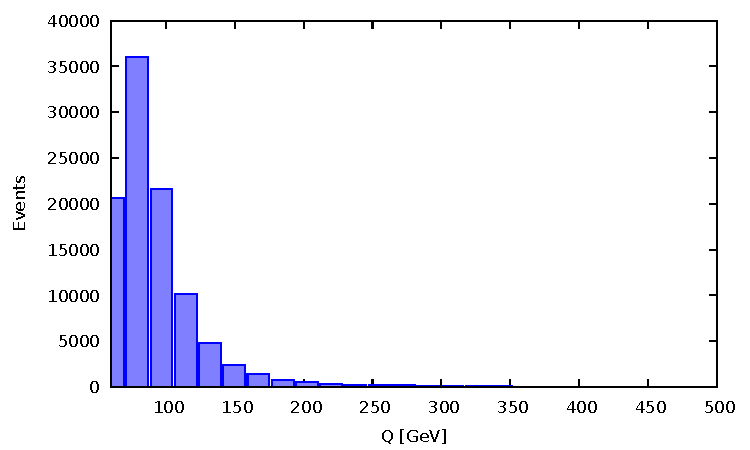
\includegraphics[width=0.49\linewidth]{./res/gfx/Q-colsim.pdf}
  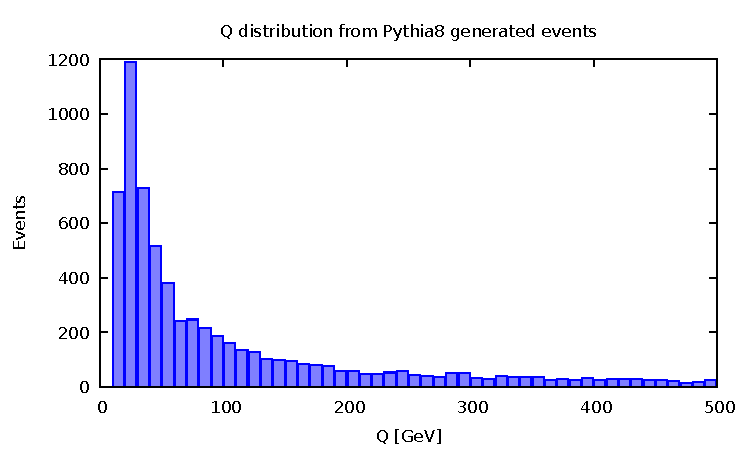
\includegraphics[width=0.49\linewidth]{./res/gfx/Q-pythia.pdf}
  \caption{Comparison between parton showering invariant masses between \textsc{ColSim}(left) and \textsc{Pythia8}(right).}
  \label{fig:Q}
\end{figure}

In Figure~\ref{fig:Q} I have given the plots for the distributions of the invariant mass for the generated events. There are some discrepancies, most notably, \textsc{Pythia8} contains some additional events in the higher $Q$ range. Figure~\ref{fig:y} contains the rapidity distributions for the generated events (rapidity is a measure of speed, roughly speaking). In my code, this value is normalized a bit differently, but we notice that it follows the same pattern, i.e. higher (absolute value of) rapidity events are less likely. Lastly, in Figure~\ref{fig:x1} are the momentum fractions the quark in the initial reaction contains. These are remarkably equivalent; evidently, the quarks involved in the showering process represent those with a small momentum fraction in the proton.


\begin{figure}[ht]
  \centering
  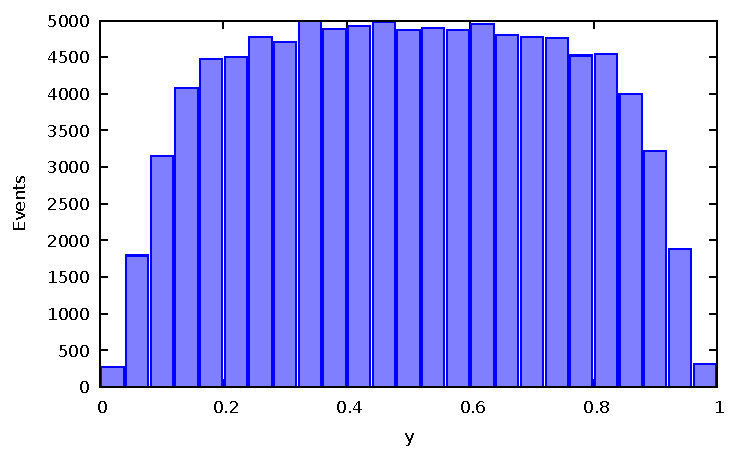
\includegraphics[width=0.49\linewidth]{./res/gfx/y-colsim.pdf}
  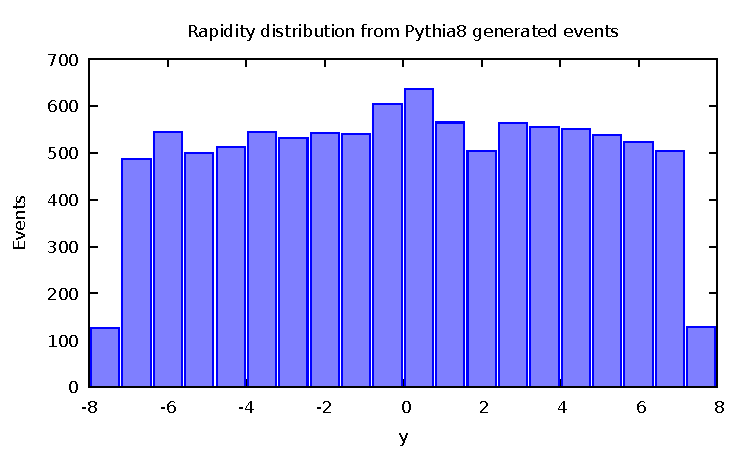
\includegraphics[width=0.49\linewidth]{./res/gfx/y-pythia.pdf}
  \caption{Comparison between rapidity between \textsc{ColSim}(left) and \textsc{Pythia8}(right).}
  \label{fig:y}
\end{figure}

\begin{figure}[ht]
  \centering
  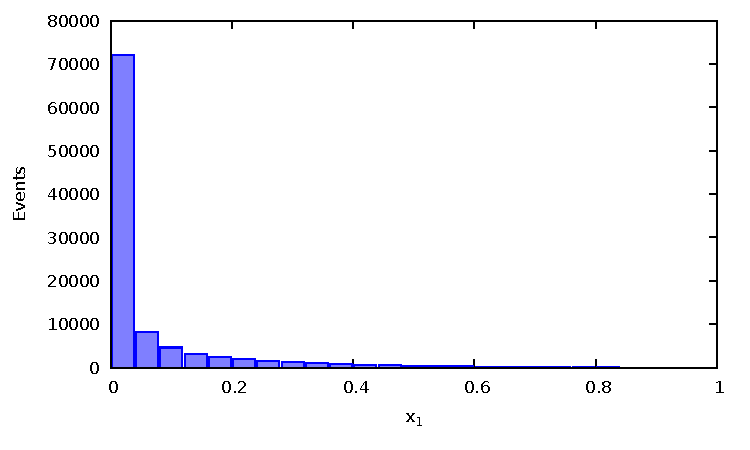
\includegraphics[width=0.49\linewidth]{./res/gfx/x1-colsim.pdf}
  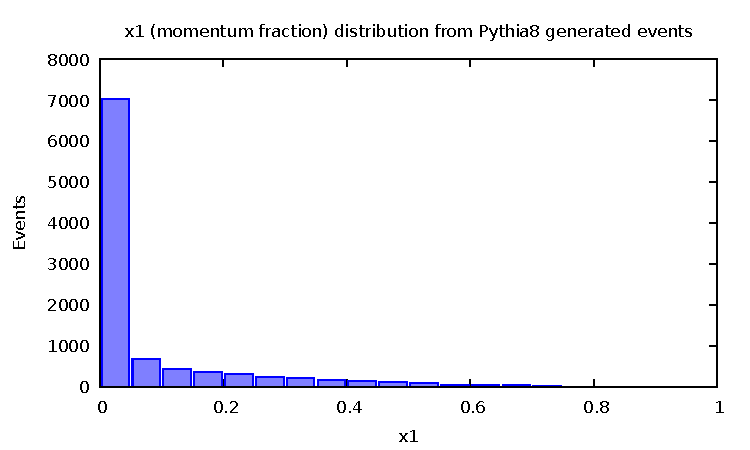
\includegraphics[width=0.49\linewidth]{./res/gfx/x1-pythia.pdf}
  \caption{Comparison between the momentum fraction between \textsc{ColSim}(left) and \textsc{Pythia8}(right).}
  \label{fig:x1}
\end{figure}



\subsection{Face Validation}

My understanding of this section is that half of it is meant to be comparing the model outputs with what is expected by field experts. Of course, if my model matches the behavior both quantitatively in the case of the cross section calculation and quantitatively in terms of the parton showering, and the comparisons are drawn between programs written by field experts, then I have more or less already satisfied the requirements for this section.

Further, a few implementation specifics have been done with assistance from a particle theorist here at KSU who specializes in Monte Carlo algorithms and event generators. I have nothing to cite in this regard, but considering again that the behavior of the model matches so well with current literature and existing models I think that I have satisfied this section.



\subsection{Historical Validation}

In the case of my model, there is not much of a reason to compare with historical data. In principle, the results themselves have not drastically changed, but rather our computational tools and theories have grown to more or less reduce the error/uncertainty with the actual calculation of values. For instance, the value of all the input parameters have more or less remained the same since their conception, but have simply had their uncertainty reduced. All I'd be doing, then, is comparing against results that effectively represent the incomplete theory and incomplete computational results, which is not instructive.


\subsection{Follow-up from Milestone 6}

In general, the performance of the model under the variation of the possible input parameters was great. The only item that was slightly suspicious at the time was the fact that a moderately significant increase of the center of mass energy led to only a small shift in the curve of the transverse momentum of the generated events for the hard scattering process. After consideration, this is not very surprising: the center-of-mass energy is related to the \textit{longitudinal} motion of the protons along the beam axis and hence the quarks. However, we were measuring the \textit{transverse} momentum, which is perpendicular to the beam axis. Therefore, an increase in the center-of-mass energy of the quarks doesn't lead to a \textit{direct} increase in the transverse momentum since the two planes are perpendicular, but should increase it a \textit{little} simply due to an excess of energy in the collision; it should be more likely to create particles of higher transverse momentum, but the small shift is much more reasonable and not something to be worried about.

Apart from that output, there is nothing else to discuss regarding the performance of the model from the previous milestone.






%%% Local Variables:
%%% mode: LaTeX
%%% TeX-master: "../../Milestone7"
%%% End:
